%\VignetteIndexEntry{RADseq_Tools_tutorial}
\documentclass{article}
\usepackage{Sweave}
\usepackage[utf8x]{inputenc} 
\title{A Tutorial for RADseq_Tools}
\author{Angel Rivera-Colon & Kira Long}
\setlength{\parindent}{0pt}

\begin{document}

\Sconcordance{concordance:Tutorial_for_RADseq_Tools.tex:Tutorial_for_RADseq_Tools.Rnw:%
1 27 1 1 2 7 0 1 2 3 1 1 2 4 0 1 2 1 1 1 2 4 0 1 2 1 1 1 2 4 0 1 2 10 1 %
1 2 4 0 2 2 1 0 1 2 11 0 1 2 2 1 1 2 4 0 1 2 1 1 1 2 1 0 1 2 22 0 1 2 %
23 1 1 4 18 0 2 2 5 0 1 2 3 1}



\begin{center}
\section*{\huge A Tutorial for RADseq\_Tools}
\subsection*{\Large Angel Rivera-Colon \& Kira Long}
\end{center}


\section{Introduction:}

Restriction site-Associated DNA sequencing (RADseq) is a modern genomic sequencing technique that has greatly advanced the field of population genomics. As a reduced representation-sequencing method, RADseq has decreased per-individual sequencing costs, making genome-wide studies more widely accessible to the research community (Catchen, et al. 2017). Additionally, it allows for the cost-effective sequencing and genotyping of multiple individuals, which is particularly important when discerning genetic variation in natural populations (Narum, et al. 2013). Moreover, RADseq’s compatibility with multiple genomic approaches, including phylogenomics, de novo population genomics, and genomic scans, have made it a key player in modern population genomics (Andrews, et al. 2016).\\
Although RADseq studies require relatively little previous information on the genome of interest, the selection of restriction enzymes and its subsequent effect on marker density remains one of RADseq’s limiting factors (Lowry, et al. 2017). The selection of a poor enzyme can then lead to genome undersampling, resulting in low marker density, or oversampling, affecting the resulting downstream coverage. Based on this, we developed an \texttt{R} package pipeline for the exploratory analysis of RADseq data to guide researchers in planning their study and improving data quality. \texttt{RADseq\_tools} estimates important information for the initial experimental design, including number of cutsites, and marker density and distribution for different user-defined restriction enzyme sites and reference genomes. Even when the reference of interest is not available, the user can explore with available genomes in related taxa and use this information to extrapolate the marker properties for their experiments. In addition, this package can assist with determining the cost of a RADseq experiment by providing estimates of expected coverage, number of samples per lane, and required read throughput. 


\section{Getting started:}
\subsection{Verifying R version}
To run \emph{RADseq\_Tools}, make sure you have a recent \texttt{R} installation. The package was written using \texttt{R version 3.4.2}, but should work with versions above \texttt{3.1.0}. To verify the installed \texttt{R} version, use:
\begin{Schunk}
\begin{Sinput}
> R.version.string
\end{Sinput}
\begin{Soutput}
[1] "R version 3.4.2 (2017-09-28)"
\end{Soutput}
\end{Schunk}

\subsection{Installation}
Install the \emph{RADseq\_Tools} package from \texttt{CRAN} using:

\begin{Schunk}
\begin{Sinput}
> install.packages("RADseq_Tools")
\end{Sinput}
\end{Schunk}

Load the package for use with:
\begin{Schunk}
\begin{Sinput}
> library(RADseq_Tools)
\end{Sinput}
\end{Schunk}

Alternatively, source the functions using:
\begin{Schunk}
\begin{Sinput}
> source('./../R/Functions.R')
\end{Sinput}
\end{Schunk}

Additional information on the package can be found in:\\ \texttt{https://github.com/angelgr2/radseq\_tools}


\section{Tutorial:}

This brief guide will provide examples of all the package's basic functions and arguments. It uses a test dataset available with the package. It consist of a small FASTA file containing the first 100Kb of sequence of six Three Spine Stickleback (\emph{Gasterosteus aculeatus}) chromosomes.

\subsection{Load and process reference sequence}

To begin, we need to load the reference sequence into a \texttt{RADseq\_Tools} object. This new \texttt{sequence} object can then be used to search restriction site. Create a variable containing the path to the reference sequence.  
\begin{Schunk}
\begin{Sinput}
> fasta_dir <- './../inst/extdata/test_geno.fa.gz'
\end{Sinput}
\end{Schunk}
This path variable is then the input of the \texttt{process\_fasta} function, which reads the file provided in the path, converting multi-line sequence objects into single line sequences. Sequences bellow 10kb are filtered and not included in the resulting sequences object. The output of the function is a vector containing the sequences strings for each of the chromosomes/scaffofds in the FASTA file. Here, we are creating the object \texttt{mySeqs} using the output of \textt{process\_fasta}, and displaying the first few nucleotides for each of the chromosomes. 
\begin{Schunk}
\begin{Sinput}
> mySeqs <- process_fasta(fasta_dir, 10000)
> substr(mySeqs, 1, 60)
\end{Sinput}
\begin{Soutput}
[1] "CTCTTTGTTTTCAGGTGTGGAATGTGCTTTCTACCACGGCTACAAATACTACAAAGGATG"
[2] "TGACTATTAAGGCGTTTGCAGGCTGAGAGAAGCCAGTCTTGAATGCTACCCCCTTTTGAG"
[3] "GCTAGCCTGTTTAAACCAAACCATCGGTGTGTATGATTACTTGCGCCCACACCCGGTCTC"
[4] "GTATTATATAGTAAATACTATACATTTTCTCTACAGATAGTACAGTGAGTTTACTCTACA"
[5] "GCTAATATTTTTATGGCTGAGTGGGAGGATTCAGTCCTGAAAATGTGTCCTAAAAAACCA"
[6] "AACCCATCGCCTTATAGGCTGTACTTTATCCTCCAATGATGGAGCAGTTCTCCGCTGCGC"
\end{Soutput}
\end{Schunk}

\subsection{Find restriction sites in the reference sequences}
The first part of finding the restriction cutsite position is defining the query to be searched, the sequence of the restriction enzyme. In this example, we are using the enzyme \texttt{SbfI}, which cuts at the sequence \texttt{CCTGCAGG}.
\begin{Schunk}
\begin{Sinput}
> SbfI <- 'CCTGCAGG'
\end{Sinput}
\end{Schunk}
Once the restriction site sequence is defined, it will be searched in the stored sequences using the \texttt{find\_cuts} function. Using \texttt{gregexpr}, it will find all matches of the restriction site query in the reference sequences. The resulting output is a list of vectors, containing all the per-chromosome/scaffold match positions.
\bigbreak
Here, we see the cutsite position for the first three test sequences:

\begin{Schunk}
\begin{Sinput}
> myCuts <- find_cuts(mySeqs, SbfI)
> myCuts[c(1,2,3)]
\end{Sinput}
\begin{Soutput}
[[1]]
[1] 11812 33253 49707 65489 65747 65834 67213 89247 92064

[[2]]
[1]   330 37897 75355 89527

[[3]]
[1]  3941 15515 28777 40042 47416 63187 70615 98324
\end{Soutput}
\end{Schunk}

\subsection{Find cutsite distribution}
After determining the position of the cutsites, it is also important to determine the distribution of cutsite in the genome, as it gives us an idea of the number of cutsites and the average inter-cutsite distance. The distribution can be calculated using the \texttt{cutsite\_distance} function. Using the cutsite position list resulting from the \texttt{find\_cuts} function, it will output a single vector containing the inter-cutsite distance for all cutsites in the genome.
\begin{Schunk}
\begin{Sinput}
> cutDist <- cutsite_distance(myCuts)
> cutDist[1:10]
\end{Sinput}
\begin{Soutput}
 [1] 11812 21441 16454 15782   258    87  1379 22034  2817   330
\end{Soutput}
\end{Schunk}
The resulting vector is compatible with all of \texttt{R} vector function, thus other statistical measures can be obtained. For example:
\begin{Schunk}
\begin{Sinput}
> summary(cutDist)
\end{Sinput}
\begin{Soutput}
   Min. 1st Qu.  Median    Mean 3rd Qu.    Max. 
     87    3098   10863   12603   15733   69883 
\end{Soutput}
\begin{Sinput}
> hist(cutDist, xlab='Distance (bp)', 
+      ylab='Frequency', main='Cutsite distance distribution' )
\end{Sinput}
\end{Schunk}
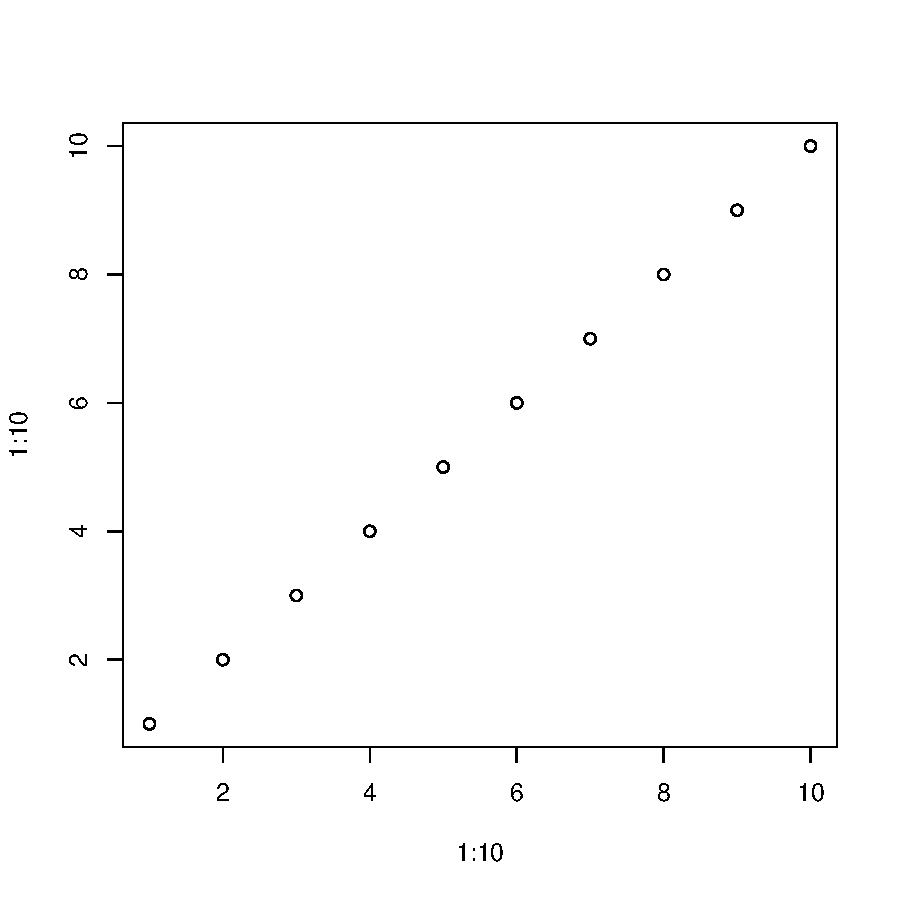
\includegraphics{Tutorial_for_RADseq_Tools-010}

\subsection{Find number of cutsites}
In addition to finding the inter-cutsite distance distribution, we can also determine the total number of cutsites using the \texttt{number\_cutsites} functions. It takes as input the original cutiste positions object product of the \texttt{find\_cuts} function, and outputs a single numeric value.
\begin{Schunk}
\begin{Sinput}
> nCuts <- number_cutsites(myCuts)
> nCuts
\end{Sinput}
\begin{Soutput}
[1] 42
\end{Soutput}
\end{Schunk}
Alternatively, the number of cutsites can be manually calculated from the length of the cutsite distribution object.
\begin{Schunk}
\begin{Sinput}
> length(cutDist)
\end{Sinput}
\begin{Soutput}
[1] 42
\end{Soutput}
\end{Schunk}

\subsection{Estimate per-sample coverage}
Using the estimations of cutsite distribution, the user can estimate the expected per-sample coverage when running a sequencing experiment using the \texttt{Per\_Sample\_Coverage} function. The function requires a number of cutsites (likely calculated with the \texttt{number\_cutsites} function), number of samples and the type of sequencing machine used, either Illumina HiSeq2500 (\texttt{'hiseq2500'}) or HiSeq4000 (\texttt{'hiseq4000'}) with their corresponding read throughput. The output is a vector contaning the extimated per-sample coverage for the machine's low, medium and high read throughput. 
\begin{Schunk}
\begin{Sinput}
> nCuts <- 35000
> nSams <- 96
> illumina <- 'hiseq2500'
> Per_Sample_Coverage(nCuts, nSams, illumina)
\end{Sinput}
\begin{Soutput}
  Low   Med    Hi 
32.74 46.13 59.52 
\end{Soutput}
\begin{Sinput}
> illumina <- 'hiseq4000'
> Per_Sample_Coverage(nCuts, nSams, illumina)
\end{Sinput}
\begin{Soutput}
  Low   Med    Hi 
 74.4 111.6 148.8 
\end{Soutput}
\end{Schunk}









\section{Other applications:}
\section{References:}


Andrews, K. R., Good, J. M., Miller, M. R., Luikart, G., \& Hohenlohe, P. A. (2016). Harnessing the power of RADseq for ecological and evolutionary genomics. \emph{Nature Reviews. Genetics}, 17(2), 81–92. doi.org/10.1038/nrg.2015.28

Catchen, J. M., Hohenlohe, P. A., Bernatchez, L., Funk, W. C., Andrews, K. R. and Allendorf, F. W. (2017), Unbroken: RADseq remains a powerful tool for understanding the genetics of adaptation in natural populations. \emph{Mol Ecol Resour}, 17: 362–365. doi:10.1111/1755-0998.12669

Lowry DB, Hoban S, Kelley JL, et al. (2017). Responsible RAD: Striving for best practices in population genomic studies of adaptation. \emph{Mol Ecol Resour}. 17:366–369. doi.org/10.1111/1755-0998.12677

Narum, S. R., Buerkle, C. A., Davey, J. W., Miller, M. R. and Hohenlohe, P. A. (2013), Genotyping-by-sequencing in ecological and conservation genomics. \emph{Molecular Ecology}, 22: 2841–2847. doi: 10.1111/mec.12350









Hello, this is a test. 
\begin{Schunk}
\begin{Sinput}
> for(i in 1:10){
+   print(i)
+ }
\end{Sinput}
\begin{Soutput}
[1] 1
[1] 2
[1] 3
[1] 4
[1] 5
[1] 6
[1] 7
[1] 8
[1] 9
[1] 10
\end{Soutput}
\end{Schunk}
This is a plot
\begin{Schunk}
\begin{Sinput}
> plot(1:10,1:10)
\end{Sinput}
\end{Schunk}
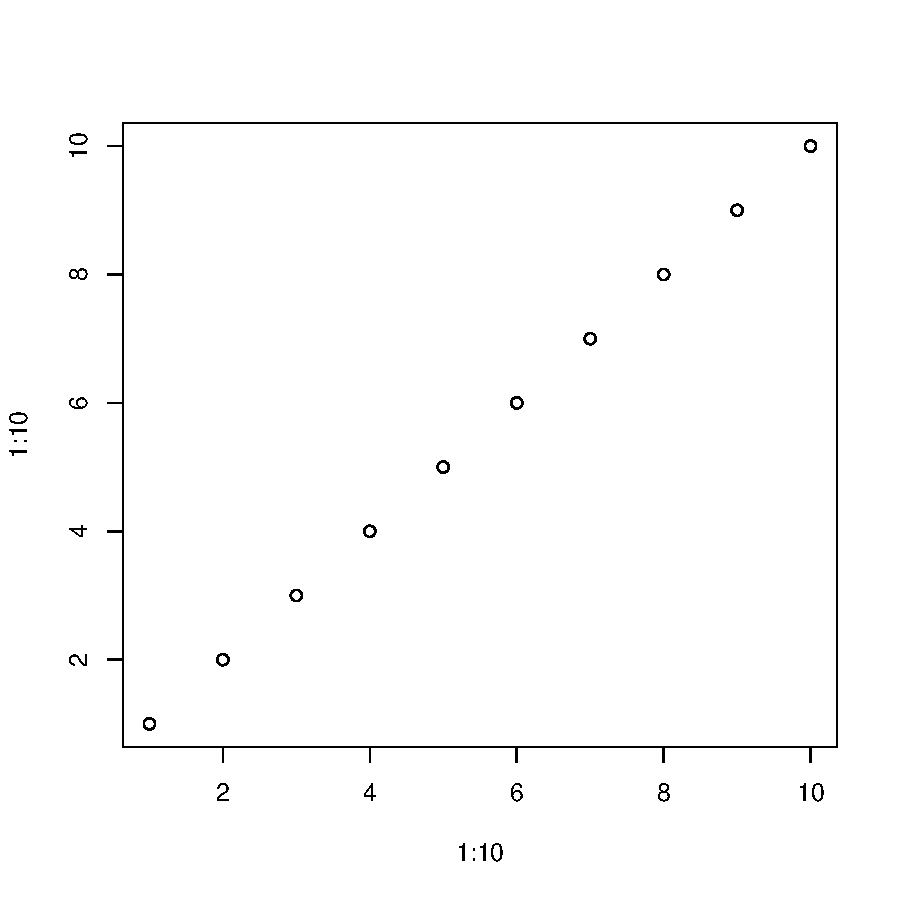
\includegraphics{Tutorial_for_RADseq_Tools-015}



\end{document}
